\documentclass{standalone}
\usepackage{tikz}
\usetikzlibrary{patterns, positioning}
\usepackage[sfdefault]{ClearSans} %% option 'sfdefault' activates Clear Sans as the default text font
\usepackage[T1]{fontenc}

\begin{document}
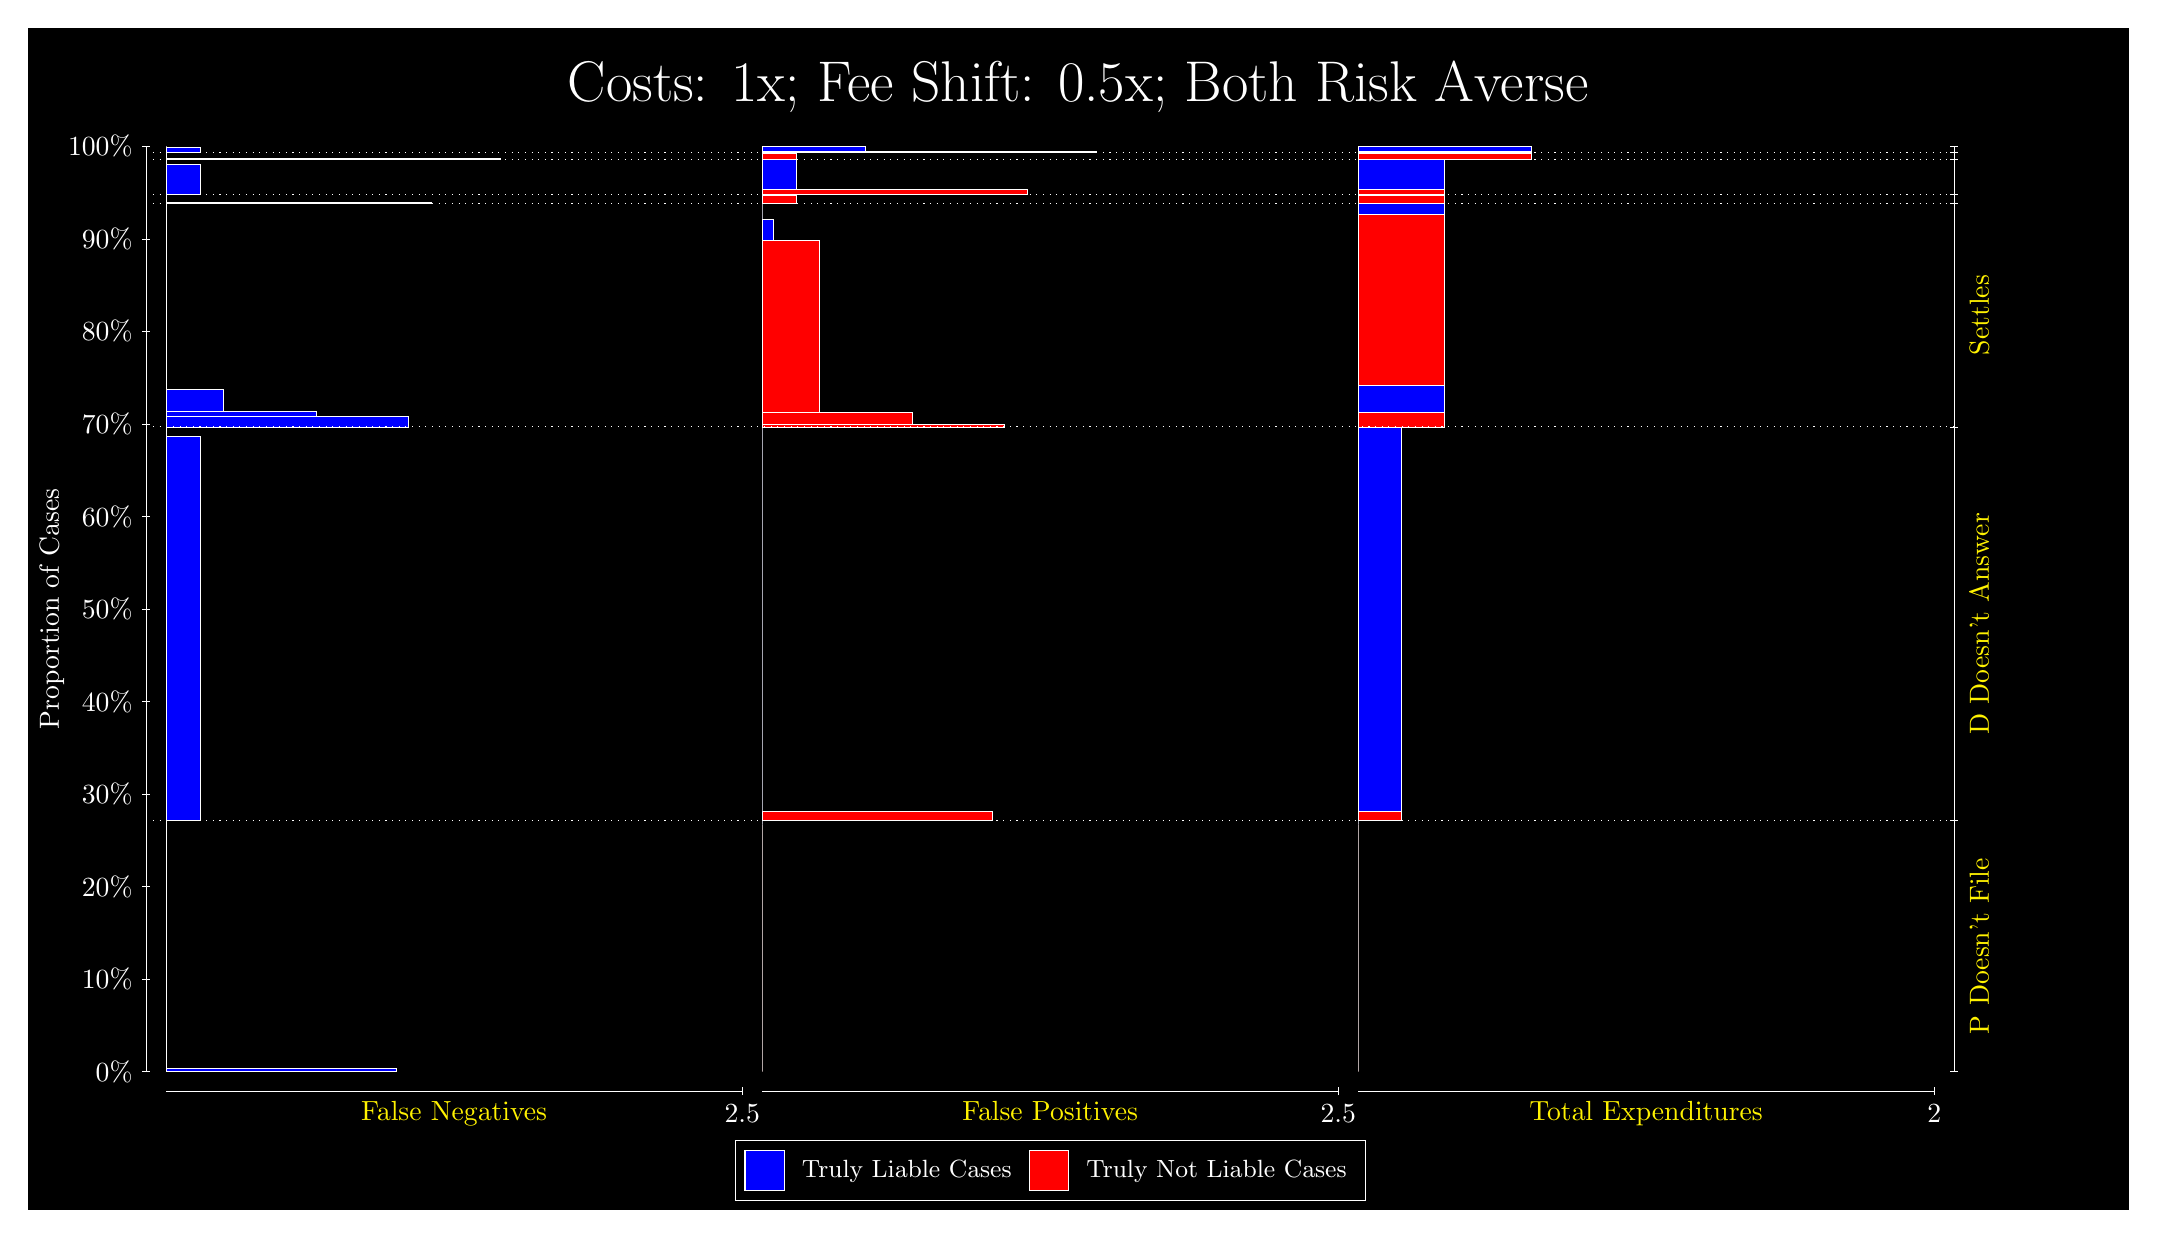
\begin{tikzpicture}
\draw[fill=black] (0,0) rectangle (26.667,15);
\draw[text=white] (0,13.5) rectangle (26.667,15) node[midway] {\huge Costs: 1x; Fee Shift: 0.5x; Both Risk Averse};
\draw[white, very thin] (1.5,1.75) -- (1.5,13.5);
\node[rotate=90, text=white, anchor=center] at (0.3, 7.625) {Proportion of Cases};
\draw[white, very thin] (1.45,1.75) -- (1.55,1.75);
\node[text=white, anchor=east] at (1.45, 1.75) {0\%};
\draw[white, very thin] (1.45,2.925) -- (1.55,2.925);
\node[text=white, anchor=east] at (1.45, 2.925) {10\%};
\draw[white, very thin] (1.45,4.1) -- (1.55,4.1);
\node[text=white, anchor=east] at (1.45, 4.1) {20\%};
\draw[white, very thin] (1.45,5.275) -- (1.55,5.275);
\node[text=white, anchor=east] at (1.45, 5.275) {30\%};
\draw[white, very thin] (1.45,6.45) -- (1.55,6.45);
\node[text=white, anchor=east] at (1.45, 6.45) {40\%};
\draw[white, very thin] (1.45,7.625) -- (1.55,7.625);
\node[text=white, anchor=east] at (1.45, 7.625) {50\%};
\draw[white, very thin] (1.45,8.8) -- (1.55,8.8);
\node[text=white, anchor=east] at (1.45, 8.8) {60\%};
\draw[white, very thin] (1.45,9.975) -- (1.55,9.975);
\node[text=white, anchor=east] at (1.45, 9.975) {70\%};
\draw[white, very thin] (1.45,11.15) -- (1.55,11.15);
\node[text=white, anchor=east] at (1.45, 11.15) {80\%};
\draw[white, very thin] (1.45,12.325) -- (1.55,12.325);
\node[text=white, anchor=east] at (1.45, 12.325) {90\%};
\draw[white, very thin] (1.45,13.5) -- (1.55,13.5);
\node[text=white, anchor=east] at (1.45, 13.5) {100\%};

\draw[white, very thin] (24.457,1.75) -- (24.457,13.5);
\draw[white, very thin] (24.407,1.75) -- (24.507,1.75);
\node[anchor=west] at (24.407, 1.75) {};
\draw[white, very thin] (24.407,4.935) -- (24.507,4.935);
\node[anchor=west] at (24.407, 4.935) {};
\draw[white, very thin] (24.407,9.9375) -- (24.507,9.9375);
\node[anchor=west] at (24.407, 9.9375) {};
\draw[white, very thin] (24.407,12.778) -- (24.507,12.778);
\node[anchor=west] at (24.407, 12.778) {};
\draw[white, very thin] (24.407,12.888) -- (24.507,12.888);
\node[anchor=west] at (24.407, 12.888) {};
\draw[white, very thin] (24.407,13.333) -- (24.507,13.333);
\node[anchor=west] at (24.407, 13.333) {};
\draw[white, very thin] (24.407,13.422) -- (24.507,13.422);
\node[anchor=west] at (24.407, 13.422) {};
\draw[white, very thin] (24.407,13.5) -- (24.507,13.5);
\node[anchor=west] at (24.407, 13.5) {};

\draw[white, very thin, fill=blue] (1.75,1.75) rectangle (4.6775,1.7951);
\draw[white, very thin, fill=red] (1.75,1.7951) rectangle (1.75,4.935);
\draw[white, very thin, fill=blue] (1.75,4.935) rectangle (2.1891,9.8197);
\draw[white, very thin, fill=red] (1.75,9.8197) rectangle (1.75,9.9375);
\draw[white, very thin, fill=blue] (1.75,9.9375) rectangle (4.8239,10.075);
\draw[white, very thin, fill=blue] (1.75,10.075) rectangle (3.6529,10.141);
\draw[white, very thin, fill=blue] (1.75,10.141) rectangle (2.4819,10.41);
\draw[white, very thin, fill=red] (1.75,10.41) rectangle (1.75,12.778);
\draw[white, very thin, fill=blue] (1.75,12.778) rectangle (5.1167,12.791);
\draw[white, very thin, fill=red] (1.75,12.791) rectangle (1.75,12.888);
\draw[white, very thin, fill=blue] (1.75,12.888) rectangle (2.1891,13.271);
\draw[white, very thin, fill=red] (1.75,13.271) rectangle (1.75,13.333);
\draw[white, very thin, fill=blue] (1.75,13.333) rectangle (5.9949,13.346);
\draw[white, very thin, fill=red] (1.75,13.346) rectangle (1.75,13.422);
\draw[white, very thin, fill=blue] (1.75,13.422) rectangle (2.1891,13.486);
\draw[white, very thin, fill=red] (1.75,13.486) rectangle (1.75,13.5);
\draw[white, very thin, fill=red] (9.3189,1.75) rectangle (9.3189,4.8899);
\draw[white, very thin, fill=blue] (9.3189,4.8899) rectangle (9.3189,4.935);
\draw[white, very thin, fill=red] (9.3189,4.935) rectangle (12.246,5.0528);
\draw[white, very thin, fill=blue] (9.3189,5.0528) rectangle (9.3189,9.9375);
\draw[white, very thin, fill=red] (9.3189,9.9375) rectangle (12.393,9.9669);
\draw[white, very thin, fill=red] (9.3189,9.9669) rectangle (11.222,10.124);
\draw[white, very thin, fill=red] (9.3189,10.124) rectangle (10.051,12.306);
\draw[white, very thin, fill=blue] (9.3189,12.306) rectangle (9.4652,12.574);
\draw[white, very thin, fill=blue] (9.3189,12.574) rectangle (9.3189,12.778);
\draw[white, very thin, fill=red] (9.3189,12.778) rectangle (9.758,12.875);
\draw[white, very thin, fill=blue] (9.3189,12.875) rectangle (9.3189,12.888);
\draw[white, very thin, fill=red] (9.3189,12.888) rectangle (12.686,12.95);
\draw[white, very thin, fill=blue] (9.3189,12.95) rectangle (9.758,13.333);
\draw[white, very thin, fill=red] (9.3189,13.333) rectangle (9.758,13.41);
\draw[white, very thin, fill=blue] (9.3189,13.41) rectangle (9.3189,13.422);
\draw[white, very thin, fill=red] (9.3189,13.422) rectangle (13.564,13.436);
\draw[white, very thin, fill=blue] (9.3189,13.436) rectangle (10.636,13.5);
\draw[white, very thin, fill=red] (16.888,1.75) rectangle (16.888,4.8899);
\draw[white, very thin, fill=blue] (16.888,4.8899) rectangle (16.888,4.935);
\draw[white, very thin, fill=red] (16.888,4.935) rectangle (17.437,5.0528);
\draw[white, very thin, fill=blue] (16.888,5.0528) rectangle (17.437,9.9375);
\draw[white, very thin, fill=red] (16.888,9.9375) rectangle (17.986,10.124);
\draw[white, very thin, fill=blue] (16.888,10.124) rectangle (17.986,10.459);
\draw[white, very thin, fill=red] (16.888,10.459) rectangle (17.986,12.64);
\draw[white, very thin, fill=blue] (16.888,12.64) rectangle (17.986,12.778);
\draw[white, very thin, fill=red] (16.888,12.778) rectangle (17.986,12.875);
\draw[white, very thin, fill=blue] (16.888,12.875) rectangle (17.986,12.888);
\draw[white, very thin, fill=red] (16.888,12.888) rectangle (17.986,12.95);
\draw[white, very thin, fill=blue] (16.888,12.95) rectangle (17.986,13.333);
\draw[white, very thin, fill=red] (16.888,13.333) rectangle (19.083,13.41);
\draw[white, very thin, fill=blue] (16.888,13.41) rectangle (19.083,13.422);
\draw[white, very thin, fill=red] (16.888,13.422) rectangle (19.083,13.436);
\draw[white, very thin, fill=blue] (16.888,13.436) rectangle (19.083,13.5);
\draw[white, dotted] (1.5,4.935) -- (24.457,4.935);
\draw[white, dotted] (1.5,9.9375) -- (24.457,9.9375);
\draw[white, dotted] (1.5,12.778) -- (24.457,12.778);
\draw[white, dotted] (1.5,12.888) -- (24.457,12.888);
\draw[white, dotted] (1.5,13.333) -- (24.457,13.333);
\draw[white, dotted] (1.5,13.422) -- (24.457,13.422);
\draw[white, very thin] (1.75,1.5) -- (9.0689,1.5);
\node[text=yellow, anchor=north] at (5.4094, 1.5) {False Negatives};
\draw[white, very thin] (9.0689,1.45) -- (9.0689,1.55);
\node[text=white, anchor=north] at (9.0689, 1.45) {2.5};

\draw[white, very thin] (9.3189,1.5) -- (16.638,1.5);
\node[text=yellow, anchor=north] at (12.978, 1.5) {False Positives};
\draw[white, very thin] (16.638,1.45) -- (16.638,1.55);
\node[text=white, anchor=north] at (16.638, 1.45) {2.5};

\draw[white, very thin] (16.888,1.5) -- (24.207,1.5);
\node[text=yellow, anchor=north] at (20.547, 1.5) {Total Expenditures};
\draw[white, very thin] (24.207,1.45) -- (24.207,1.55);
\node[text=white, anchor=north] at (24.207, 1.45) {2};

\node[text=yellow, centered, rotate=90] at (24.777, 3.3425) {P Doesn't File};
\node[text=yellow, centered, rotate=90] at (24.777, 7.4363) {D Doesn't Answer};
\node[text=yellow, centered, rotate=90] at (24.777, 11.358) {Settles};





\draw (12.978300999999998,1.5) node[draw=none] (baseCoordinate) {};
\begin{scope}[align=center]
        \matrix[scale=0.5, draw=white, below=0.5cm of baseCoordinate, nodes={draw}, column sep=0.1cm]{
            \node[rectangle, draw, minimum width=0.5cm, minimum height=0.5cm, fill=blue] {}; &
            \node[draw=none, font=\small, text=white] (B) {Truly Liable Cases}; &
            \node[rectangle, draw, minimum width=0.5cm, minimum height=0.5cm, fill=red] {}; &
            \node[draw=none, font=\small, text=white] (B) {Truly Not Liable Cases}; \\
            };
\end{scope}

\end{tikzpicture}
\end{document}